Due to the detailed planning and devolopment of the GUI elements during the first deliverable the creation of the main operations GUI elements were able to be completed rather swiftly. However there was an initial lag caused by the lack of familiarity with JavaFX and scene builder. After a few hours of familiarization, a FXML closely resembling the protoyped design was created for the main order screen. 

\begin{figure}[ht]
	\centering
	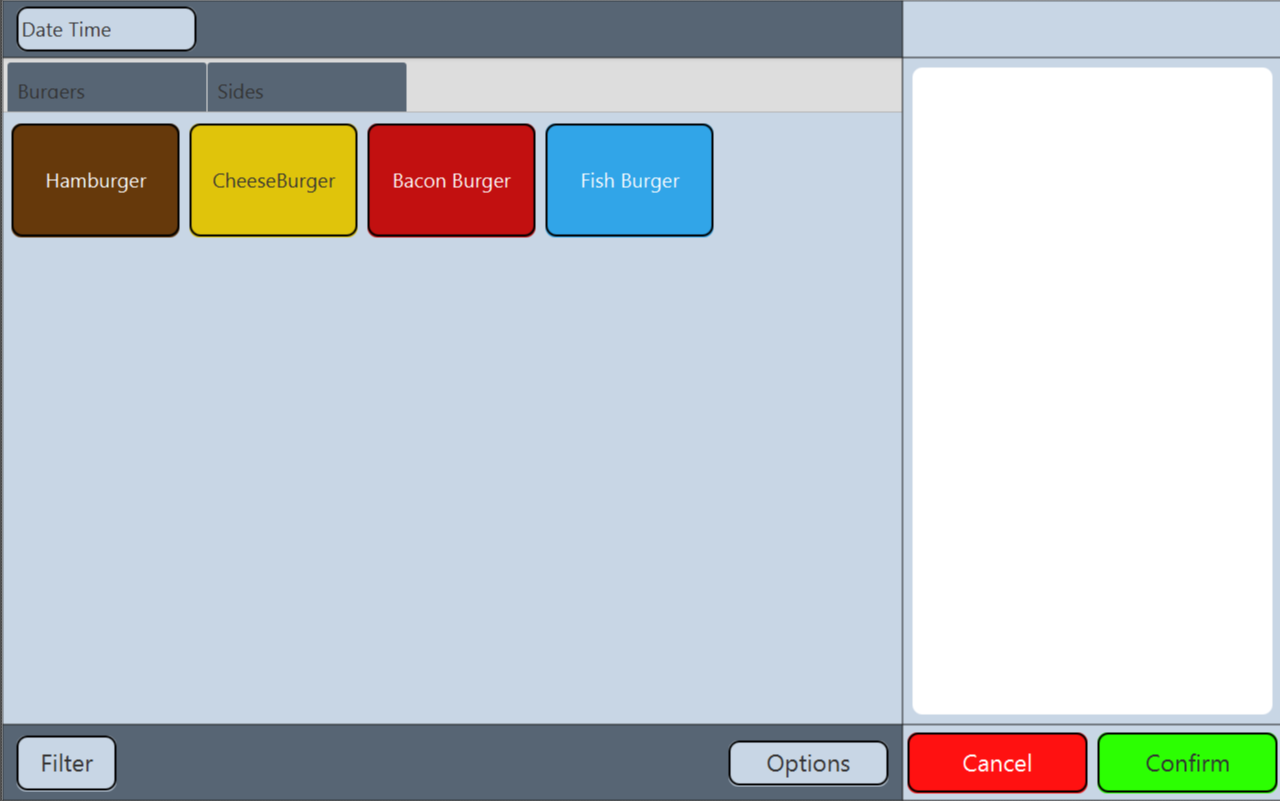
\includegraphics[width=150mm]{images/old_order_screen.png}
	\caption{Initial implimentation of the prototyped defsign}
	\label{fig:old_order_screen}
\end{figure}

Most of the differences between the first implimentation and the protoype (\ref{fig:old_order_screen} and \ref{fig:management_screen_moqueup} respectivly) can be attributed to the differences between the programs used to create them as well as constraints created when implimenting elements with relative alignments or elements that exist within other elements. 

The first implimentation of the GUI was effectivly a simple skin of the prototype with buttons that printed their name but no further functionallity. This allowed for a devolopment of basic skills and expereince as well as a platform for further devolopment moving forward. The experience gained from this base was then taken forward and used in the creation of the other UI elements for the operations side whilst refining the main order screen and adding the functionality. The creation of these scenes and their functionallity was significantly easier after getting over the initial learning curve of JavaFX and SceneBuilder.

During this time there was a converstion surrounding the implimentation of the buttons for adding items to orders. Initially the buttons were designed and implimented to all be generated as blank, disabled buttons and then be enabled and filled when needed, however we decided to switch to an approach using buttons that were dynamically created and loaded when the main order screen was loaded in an effort to reduce cluttering of the main order window (QRXX?).

Through out the devolopment of the operations side of the GUI small changes and adjustments were made to the design in an effort to clean and improve elements as they were noticed. An example of this was removing the black outline sorounding each item button. This change gave the main order screen a cleaner appearance, which was part of the driving force for the operational GUI.

The devolopment of the management side GUI were unfortuantly neglected during the planning stages so their devolopment was left more plain and focused on the function. This caused the initial management screen prototype (see \ref{fig:management_screen_moqueup}) to be paritally overhauled to a more tabular based aproach that focused on presenting information and implimenting functional elements in an efficent and simplified manner.

It is also worth noting that significant efforts towards planning and implimenting the system architecture proved extremely valuable during the implimentation of the functional elements and methods of the GUIs. This allowed for rapid implimentation of features even when under time pressures close to the devlierable deadlines. 

